% 第3章第3节：最大流与最小割（流、容量与割；残量网络；增广路径与最优性条件；Ford--Fulkerson增广法；Edmonds--Karp算法；算法分析与结果检验）。

\section{最大流与最小割}
\label{sec:graph-max-flow}

前两节各选出一个结构：一条路线或一棵树。现在设想从水厂向用户输水，每段管道有输送上限，水可以同时沿多条管道并行，也可以在中途汇合、分流。要回答的是单位时间内最多能送出多少水。这次选择的对象不是一条路径，而是每条弧上的一个流量，所有流量要同时满足容量上限和中途不积存的条件。两条路线若共用一段容量为$1$的管道，它们合计只能送$1$，不能各送$1$。

本节先建立流、容量与割，并证明任何流量都不超过任何割的容量。为了改进当前的输送方案，引入允许撤回旧流量的残量网络，由此得到判断一个流是否最优的增广路径判据，以及与之同值的割证书。随后介绍两种算法：Ford--Fulkerson方法任意选取增广路径，在整数容量下有限终止；Edmonds--Karp算法规定按最少弧数选路，对任意实容量都有与数值无关的增广次数界，并由此得到最大流最小割定理。

\subsection{流、容量与割}
\label{sec:graph-opt-flow-cut}

设$\mathcal G=(V,E)$是有限有向图，指定两个不同的顶点：源点$s$与汇点$t$。每条弧$u\to v$带有有限非负实数\emph{容量}$c_{u,v}$，表示该弧单位时间内最多能通过的量。这样的四元组$(\mathcal G,c,s,t)$称为\term{流网络}（flow network）。

\begin{definition}[流与流值]
\label{def:graph-opt-flow}
流网络上的一个\term{流}（flow）是给每条弧$u\to v$赋予实数$x_{u,v}$的一组数$\bm x=(x_{u,v})$，满足
\begin{gather}
  0\leq x_{u,v}\leq c_{u,v}\quad\text{对每条弧}\ u\to v,\label{eq:graph-opt-capacity}\\
  \sum_{u:\,u\to v}x_{u,v}=\sum_{w:\,v\to w}x_{v,w}\quad\text{对每个}\ v\in V\setminus\{s,t\}.\label{eq:graph-opt-conservation}
\end{gather}
前者称为容量约束，后者称为\term{流守恒}（flow conservation）。源点的净流出
\[
  \operatorname{val}(\bm x)=\sum_{w:\,s\to w}x_{s,w}-\sum_{u:\,u\to s}x_{u,s}
\]
称为\term{流值}（flow value）。流值最大的流称为\term{最大流}（maximum flow）。
\end{definition}

流守恒说明中间顶点只转运、不积存，所以源点送出的净量应该全部到达汇点。为验证这一点，对每个顶点计算净流出（流出减流入）并对全部顶点求和：每条弧的流量在起点算一次正、在终点算一次负，总和为零。中间顶点的净流出都是零，于是源点的净流出等于汇点的净流入，即$\operatorname{val}(\bm x)$也是$t$收到的净量。流值不是全图各弧流量的总和：一单位流量经过三条弧到达汇点，只算一单位流值。

\paragraph{割与割容量}
为了估计流值能有多大，把顶点分成包含$s$的一侧$S$与包含$t$的一侧$\bar S=V\setminus S$，称$(S,\bar S)$为一个$s$--$t$割。这里沿用第~\ref{sec:graph-opt-cut-property}节割的含义，只是额外要求源、汇分居两侧。割的\term{割容量}（cut capacity）只累计从源侧跨向汇侧的弧：
\[
  c(S,\bar S)=\sum_{u\in S,\ v\in\bar S,\ u\to v}c_{u,v}.
\]
从汇侧指回源侧的弧不计入容量。直观上，任何从$s$到$t$的输送都要穿过这个割，穿过的总量不可能超过这些弧的容量之和。下面把这一直观变成证明。

\begin{lemma}[流值不超过割容量]
\label{lem:graph-opt-weak-duality}
对任意流$\bm x$与任意$s$--$t$割$(S,\bar S)$，有
\begin{equation}
  \operatorname{val}(\bm x)=\sum_{u\in S,\,v\in\bar S}x_{u,v}-\sum_{v\in\bar S,\,u\in S}x_{v,u}\leq c(S,\bar S).
  \label{eq:graph-opt-net-flow-cut}
\end{equation}
\end{lemma}

\begin{proof}
对$S$中的全部顶点把净流出相加。$s$贡献$\operatorname{val}(\bm x)$，其余顶点都是中间顶点（$t\notin S$），贡献为零，所以和等于$\operatorname{val}(\bm x)$。另一方面，两端都在$S$内的弧在起点计正、在终点计负，相互抵消；剩下的只有跨割的弧：从$S$指向$\bar S$的弧计正，从$\bar S$指回$S$的弧计负。这就得到式~\eqref{eq:graph-opt-net-flow-cut}中的等式。再由容量约束，第一个和不超过$c(S,\bar S)$，第二个和不小于零，得到不等式。
\end{proof}

式~\eqref{eq:graph-opt-net-flow-cut}说明，流值等于跨过任意一个割的净流量，而每个割的容量都是流值的上界。图~\ref{fig:graph-opt-flow-network-cut}中，取$S=\{s,b\}$，跨出的弧$s\to a$与$b\to t$容量合计$6$，指回的弧$a\to b$不计入；所示流在这两条弧上分别送$3$与$3$，在$a\to b$上送回$1$，净流量$3+3-1=5$恰为流值，不超过割容量$6$。

\begin{figure}[!htb]
  \centering
  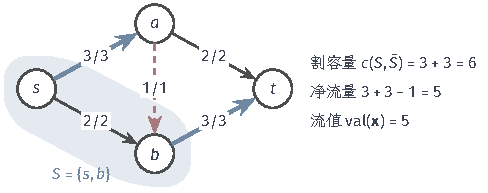
\includegraphics[width=82.564mm]{figures/01-basic-mathematics/04-graphs/tikz/c3-flow-network-cut/figure.pdf}
  \caption{流网络、流与割。弧旁的“$x/c$”表示流量与容量，每个中间顶点流入等于流出，流值为$5$。浅色底标出割的源侧$S=\{s,b\}$：跨出的弧$s\to a$、$b\to t$（蓝色粗弧）的容量计入割容量$3+3=6$；指回的弧$a\to b$（红色虚线）不计容量，其流量在净流量中扣除，$3+3-1=5$。}
  \label{fig:graph-opt-flow-network-cut}
\end{figure}

\subsection{残量网络}
\label{sec:graph-opt-residual-network}

最朴素的改进办法是：找一条从$s$到$t$、每条弧都还有剩余容量的路径，沿它多送一些。但已经选定的路线可能占用了更好的安排，只会追加流量的办法会过早卡住。下面的例子会说明这一点，补救的办法是允许撤回一部分旧流量，把撤回也当作一种可以使用的“通道”。

\paragraph{正向残量与反向残量}
给定流$\bm x$，对每条原弧$u\to v$建立两条\emph{残量弧}：正向残量弧$u\to v$，容量$c_{u,v}-x_{u,v}$，表示还能追加多少；反向残量弧$v\to u$，容量$x_{u,v}$，表示能撤回多少。只保留容量为正的残量弧，得到的有向图称为\term{残量网络}（residual network），记作$\mathcal G_{\bm x}$，残量弧的容量记作$r_{\bm x}$。例如原弧容量为$3$、当前流量为$2$时，正向残量为$1$、反向残量为$2$，如图~\ref{fig:graph-opt-residual-arc}。沿反向残量弧$v\to u$送出一单位，含义是把原弧$u\to v$上的流量减少一单位，并不要求原网络中真有一条从$v$到$u$的管道。

\begin{figure}[!htb]
  \centering
  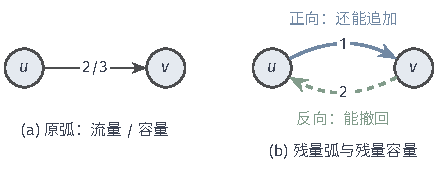
\includegraphics[width=74.186mm]{figures/01-basic-mathematics/04-graphs/tikz/c3-residual-arc/figure.pdf}
  \caption{一条原弧对应两条残量弧。(a) 原弧$u\to v$容量$3$、流量$2$。(b) 残量网络中，正向残量弧$u\to v$（蓝色）容量$3-2=1$，表示还能追加的量；反向残量弧$v\to u$（绿色虚线）容量$2$，表示能撤回的量。流量为$0$时没有反向残量弧，满流时没有正向残量弧。}
  \label{fig:graph-opt-residual-arc}
\end{figure}

\paragraph{撤回旧流的例子}
取弧$s\to a$、$s\to b$、$a\to b$、$a\to t$、$b\to t$，容量都为$1$。若先沿$s\to a\to b\to t$送一单位，三条弧都满了，剩下的$s\to b$与$a\to t$虽有空余，却连不成一条只用正向残量的$s$--$t$路径，只会追加的办法到此停止，流值为$1$。但残量网络中还有反向残量弧$b\to a$，容量$1$，于是出现路径$s\to b\to a\to t$：在$s\to b$与$a\to t$上各追加一单位，同时把$a\to b$上的流量撤回一单位。更新后的流在$s\to a$、$a\to t$、$s\to b$、$b\to t$上各为$1$，在$a\to b$上为$0$，流值为$2$。逐点核对：$a$流入$1$、流出$1$，$b$流入$1$、流出$1$，各弧都不超过容量。图~\ref{fig:graph-opt-undo-flow}画出这三个阶段。最终的实际输送是两条不相交的路线$s\to a\to t$与$s\to b\to t$，第一次选路时经过$a\to b$的那一单位被“改道”了。

\begin{figure*}[!htb]
  \centering
  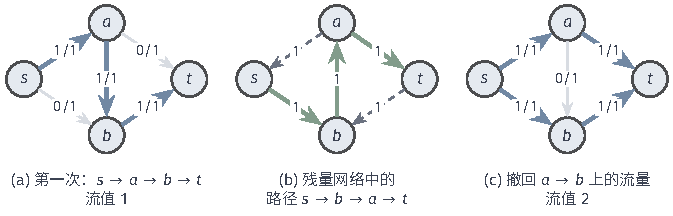
\includegraphics[width=113.901mm]{figures/01-basic-mathematics/04-graphs/tikz/c3-undo-flow/figure.pdf}
  \caption{单位容量网络中撤回旧流量。(a) 先沿$s\to a\to b\to t$送一单位（蓝色粗弧为流量$1$的弧），只用正向残量已无$s$--$t$路径。(b) 残量网络：满流弧只剩反向残量弧（灰色），绿色路径$s\to b\to a\to t$经过反向残量弧$b\to a$。(c) 沿该路径更新后，$a\to b$上的流量被撤回，流值变为$2$，实际路线为$s\to a\to t$与$s\to b\to t$。}
  \label{fig:graph-opt-undo-flow}
\end{figure*}

原网络若同时有$u\to v$与$v\to u$两条弧，残量网络中可能出现两条同向的$u\to v$残量弧：一条是原弧$u\to v$的正向残量，另一条是原弧$v\to u$的反向残量。实现时应保留每条残量弧对应哪条原弧、哪个方向的身份，沿它送流时修改的是对应原弧的流量。否则会把“真实地反向输送”与“撤回另一条弧上的流量”混成同一个量。

\subsection{增广路径与最优性条件}
\label{sec:graph-opt-augmenting-path}

有了残量网络，改进一个流的办法就统一成了找路：残量网络中的任何一条$s$--$t$路径都给出一种在不违反约束的前提下增加流值的调整。

\paragraph{增广路径与瓶颈}
残量网络$\mathcal G_{\bm x}$中从$s$到$t$的简单路径$P$称为关于$\bm x$的\term{增广路径}（augmenting path）。$P$上残量容量的最小值
\[
  \Delta=\min_{(u\to v)\in P}r_{\bm x}(u,v)>0
\]
称为$P$的\term{瓶颈容量}（bottleneck capacity）。沿$P$增广$\Delta$，是指对$P$上的每条残量弧：若它是原弧$u\to v$的正向残量，令$x_{u,v}\leftarrow x_{u,v}+\Delta$；若它是原弧$v\to u$的反向残量，令$x_{v,u}\leftarrow x_{v,u}-\Delta$。

\begin{lemma}[沿增广路径更新保持可行]
\label{lem:graph-opt-augment}
设$\bm x$是流，$P$是增广路径，瓶颈容量为$\Delta$。沿$P$增广$\Delta$后得到的$\bm x'$仍是流，并且$\operatorname{val}(\bm x')=\operatorname{val}(\bm x)+\Delta$。
\end{lemma}

\begin{proof}
容量约束：正向残量弧满足$\Delta\leq c_{u,v}-x_{u,v}$，追加后不超过容量；反向残量弧满足$\Delta\leq x_{v,u}$，撤回后不小于零。流守恒：$P$是简单路径，经过每个中间顶点$v$恰好一次，一条残量弧进入$v$，一条离开$v$。进入的那条若是正向残量，$v$的流入增加$\Delta$；若是反向残量，即撤回一条从$v$出发的原弧上的流量，$v$的流出减少$\Delta$。两种情形都使$v$的净流出减少$\Delta$。同理，离开的那条残量弧使$v$的净流出增加$\Delta$。两者相抵，$v$仍满足守恒。最后，$P$的第一条残量弧离开$s$，使$s$的净流出增加$\Delta$，而$P$是简单路径，不再回到$s$，所以流值增加$\Delta$。
\end{proof}

\paragraph{同值割证书}
引理说明，只要存在增广路径，当前流就不是最大流。反过来，没有增广路径时，能否断定当前流最大？答案是肯定的，而且可以从残量网络中直接读出一个与流值相等的割。

\begin{theorem}[增广路径判据]
\label{thm:graph-opt-augmenting-path}
设$\bm x$是流网络上的一个流，则下列三条等价：
\begin{enumerate}
  \item $\bm x$是最大流；
  \item 残量网络$\mathcal G_{\bm x}$中不存在增广路径；
  \item 存在某个$s$--$t$割$(S,\bar S)$，使$\operatorname{val}(\bm x)=c(S,\bar S)$。
\end{enumerate}
此时$(S,\bar S)$是割容量最小的$s$--$t$割，可取$S$为$\mathcal G_{\bm x}$中从$s$可达的顶点集。
\end{theorem}

\begin{proof}
由1推2：若存在增广路径，由引理~\ref{lem:graph-opt-augment}可得流值更大的流，与$\bm x$最大矛盾。

由2推3：令$S$为$\mathcal G_{\bm x}$中从$s$可达的顶点集。$s\in S$，而没有增广路径说明$t\notin S$，所以$(S,\bar S)$是$s$--$t$割。考察跨割的原弧。若$u\in S$、$v\in\bar S$且$u\to v$是原弧，则必有$x_{u,v}=c_{u,v}$，否则正向残量弧$u\to v$存在，$v$就从$s$可达了。若$v\in\bar S$、$u\in S$且$v\to u$是原弧，则必有$x_{v,u}=0$，否则反向残量弧$u\to v$存在，同样使$v$可达。把这两条代入式~\eqref{eq:graph-opt-net-flow-cut}，第一个和等于$c(S,\bar S)$，第二个和为零，故$\operatorname{val}(\bm x)=c(S,\bar S)$。

由3推1：对任意流$\bm y$，引理~\ref{lem:graph-opt-weak-duality}给出$\operatorname{val}(\bm y)\leq c(S,\bar S)=\operatorname{val}(\bm x)$，所以$\bm x$最大。同一不等式对任意割$(S',\bar S')$给出$c(S',\bar S')\geq\operatorname{val}(\bm x)=c(S,\bar S)$，所以$(S,\bar S)$的割容量最小。
\end{proof}

割容量最小的$s$--$t$割称为\term{最小割}（minimum cut）。定理把“是否最优”这个关于全部候选流的问题，化成了在残量网络中做一次遍历就能回答的问题；停止时得到的流与割互为证书，任何人都可以逐弧核对两者的数值相等，而不必相信算法本身。图~\ref{fig:graph-opt-max-flow-certificate}是第~\ref{sec:graph-opt-flow-cut}小节网络的一个最大流及其证书：残量网络中$s$的两条出弧都已满流，从$s$出发哪里也去不了，$S=\{s\}$，割容量$3+2=5$等于流值。

\begin{figure}[!htb]
  \centering
  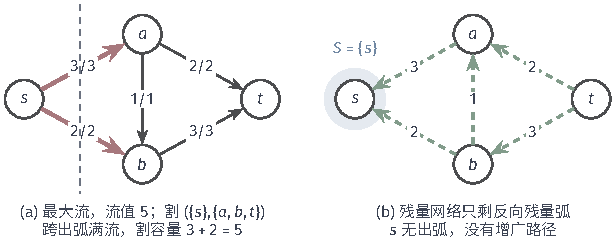
\includegraphics[width=104.186mm]{figures/01-basic-mathematics/04-graphs/tikz/c3-max-flow-certificate/figure.pdf}
  \caption{最大流与最小割互为证书。(a) 原网络上的最大流，弧旁为“流量/容量”，流值为$5$；虚线表示割$(\{s\},\{a,b,t\})$，其跨出弧$s\to a$、$s\to b$（红色）均满流，割容量$3+2=5$等于流值。(b) 对应的残量网络：五条原弧都已满流，只剩反向残量弧（绿色虚线），弧旁为残量容量；$s$没有出弧，从$s$可达的集合为$S=\{s\}$（浅色底），不存在增广路径。}
  \label{fig:graph-opt-max-flow-certificate}
\end{figure}

需要注意定理的范围。它判定一个\emph{给定}的流是否最优，并在最优时给出证书；它没有断言任意选路的增广过程一定会在有限步内走到这样的流，也还没有说明最大流一定存在。存在性由第~\ref{sec:graph-opt-edmonds-karp}小节的Edmonds--Karp算法以构造的方式补齐。

\subsection{Ford--Fulkerson增广法}
\label{sec:graph-opt-ford-fulkerson}

定理~\ref{thm:graph-opt-augmenting-path}直接给出一个算法框架：从零流出发，只要残量网络中还有增广路径就沿它增广，没有时停止。这个框架称为\term{Ford--Fulkerson方法}（Ford--Fulkerson method）。称它为“方法”，是因为它没有规定选哪条增广路径。

\begin{algorithm}[Ford--Fulkerson增广法]
\label{alg:graph-opt-ford-fulkerson}
输入：流网络$(\mathcal G,c,s,t)$。输出：流$\bm x$与割$(S,\bar S)$。状态：各原弧的流量、由流量确定的正反残量、搜索用的前驱与当前流值。
\begin{enumerate}
  \item 令$\bm x=\bm 0$。
  \item 在当前残量网络中搜索一条$s$--$t$路径，记录前驱；若没有，转第4步。
  \item 沿前驱恢复路径$P$，求瓶颈$\Delta$，按引理~\ref{lem:graph-opt-augment}更新对应原弧的流量，流值加$\Delta$，回到第2步。
  \item 令$S$为最后一次搜索中从$s$可达的顶点集，输出$\bm x$与$(S,\bar S)$。
\end{enumerate}
\end{algorithm}

每次更新都会改变若干残量：正向残量减少，反向残量增加，有的残量弧消失，也有新的出现。所以每轮都要在更新后的残量网络中重新搜索，不能沿用上一轮找到的其他路径。

\paragraph{算例}
回到图~\ref{fig:graph-opt-flow-network-cut}的网络，弧$s\to a$、$s\to b$、$a\to b$、$a\to t$、$b\to t$的容量依次为$3,2,1,2,3$。从零流出发：
\begin{enumerate}
  \item 沿$s\to a\to t$增广，瓶颈$\min\{3,2\}=2$，流值为$2$；
  \item 沿$s\to b\to t$增广，瓶颈$\min\{2,3\}=2$，流值为$4$；
  \item 此时$s\to a$剩余$1$，$a\to t$已满，沿$s\to a\to b\to t$增广，瓶颈$\min\{1,1,1\}=1$，流值为$5$。
\end{enumerate}
所得流在五条弧上依次为$3,2,1,2,3$，每条弧都满流。$a$流入$3$、流出$1+2=3$，$b$流入$2+1=3$、流出$3$，守恒成立。残量网络中$s$的两条出弧都已饱和，搜索停止，得到$S=\{s\}$，即图~\ref{fig:graph-opt-max-flow-certificate}中的证书。前面的单位容量例子也是这个框架的一次运行：先选了$s\to a\to b\to t$，第二轮的增广路径$s\to b\to a\to t$经过反向残量弧，撤回了旧的流量。

\paragraph{整数容量下的有限终止}
框架是否总会停止？容量都是整数时，答案是肯定的。

\begin{theorem}[整数容量下的有限终止]
\label{thm:graph-opt-integer-termination}
若所有容量都是非负整数，则Ford--Fulkerson方法无论怎样选择增广路径，至多经过$C_s=\sum_{w:\,s\to w}c_{s,w}$次增广就停止，输出的流是最大流，并且每条弧上的流量都是整数。
\end{theorem}

\begin{proof}
对增广次数归纳可知，流量始终是整数：零流是整数的；若当前流量都是整数，则残量$c_{u,v}-x_{u,v}$与$x_{u,v}$都是整数，瓶颈$\Delta$是正整数，更新后流量仍为整数。于是每次增广使流值至少增加$1$。另一方面，由引理~\ref{lem:graph-opt-weak-duality}，取$S=\{s\}$可知流值不超过$C_s$。所以增广至多$C_s$次。停止时没有增广路径，由定理~\ref{thm:graph-opt-augmenting-path}，所得流最大。
\end{proof}

这个定理同时说明，整数容量的网络存在每条弧流量都为整数的最大流，第~\ref{sec:graph-matching}节的匹配会用到这一点。容量为有理数时，乘以公分母即化为整数情形。但对一般的实容量，上面的整数步长论证不能照搬：每次流值都增加，增加量却可能越来越小。已知存在容量含无理数的网络，任意选路的Ford--Fulkerson方法可以永不停止，流值甚至收敛到小于最大流值的数。因此，任意选路的框架不自动具有有限终止的保证，需要对选路规则加以限制。

\subsection{Edmonds--Karp算法}
\label{sec:graph-opt-edmonds-karp}

Edmonds--Karp算法保留残量网络与增广更新，只对选路加一条规则：每次用广度优先遍历寻找弧数最少的增广路径。这里的“最短”按残量弧的条数计算，容量不参与路径长短的比较。

\begin{algorithm}[Edmonds--Karp算法]
\label{alg:graph-opt-edmonds-karp}
与算法~\ref{alg:graph-opt-ford-fulkerson}相同，只是第2步固定用第~\ref{sec:graph-bfs}节的广度优先遍历在残量网络中从$s$搜索，所得前驱路径是弧数最少的$s$--$t$路径。
\end{algorithm}

\paragraph{算例}
在同一个$3,2,1,2,3$网络上按字母顺序访问邻居，记$h(v)$为$v$在当前残量网络中的广度优先层数，即从$s$出发的最少弧数。第$1$轮，各层为$h(a)=h(b)=1$、$h(t)=2$，选出$s\to a\to t$，瓶颈$2$。第$2$轮，残量网络中$s\to a$剩$1$、$a\to t$已满，层数仍为$h(a)=h(b)=1$、$h(t)=2$，选出$s\to b\to t$，瓶颈$2$。第$3$轮，$s\to b$已满，$b$只能经$a$到达，层数变为$h(a)=1$、$h(b)=2$、$h(t)=3$，选出$s\to a\to b\to t$，瓶颈$1$。第$4$轮从$s$出发不能到达任何顶点，停止，流值为$5$。图~\ref{fig:graph-opt-edmonds-karp-layers}画出各轮的残量网络与分层。

\begin{figure*}[!htb]
  \centering
  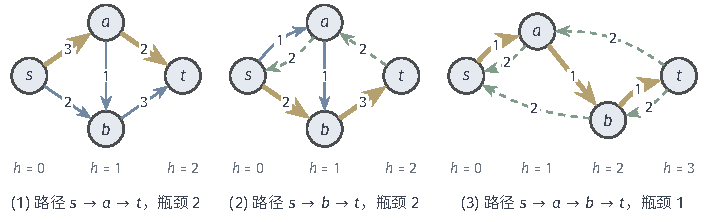
\includegraphics[width=119.567mm]{figures/01-basic-mathematics/04-graphs/tikz/c3-edmonds-karp-layers/figure.pdf}
  \caption{Edmonds--Karp算法在$3,2,1,2,3$网络上的三轮增广。每个面板是该轮开始时的残量网络，顶点按广度优先层数$h$从左到右排列，弧旁为残量容量，蓝色为正向残量弧，绿色虚线为反向残量弧；黄色粗箭头是本轮选出的弧数最少的增广路径。汇点层数依次为$2,2,3$，不随增广而减小。}
  \label{fig:graph-opt-edmonds-karp-layers}
\end{figure*}

这个网络上，Edmonds--Karp算法选出的路径恰好与前面手工选择的相同。差别在单位容量的例子中显现：任意选路时可以先选三条弧的$s\to a\to b\to t$，随后不得不撤回；Edmonds--Karp算法第一轮只会选两条弧的$s\to a\to t$，第二轮选$s\to b\to t$，两次增广即达到流值$2$，不需要撤回。

\paragraph{层数不下降}
增广次数的上界来自层数的变化。记$h_{\bm x}(v)$为$v$在$\mathcal G_{\bm x}$中从$s$出发的最少弧数，不可达时为$+\infty$。首先证明，沿最短增广路径增广不会让任何顶点离$s$更近。

\begin{lemma}[残量层数单调不减]
\label{lem:graph-opt-levels-monotone}
设$\bm x'$由$\bm x$沿$\mathcal G_{\bm x}$中一条弧数最少的增广路径增广得到，则对每个顶点$v$都有$h_{\bm x'}(v)\geq h_{\bm x}(v)$。
\end{lemma}

\begin{proof}
假设结论不成立，在所有满足$h_{\bm x'}(v)<h_{\bm x}(v)$的顶点中取$h_{\bm x'}(v)$最小的一个$v$。显然$v\neq s$。取$\mathcal G_{\bm x'}$中一条$s$到$v$的最短路径，设其最后一条弧为$u\to v$，则$h_{\bm x'}(u)=h_{\bm x'}(v)-1$；由$v$的最小性，$h_{\bm x'}(u)\geq h_{\bm x}(u)$。分两种情形。

若弧$u\to v$在增广前已在$\mathcal G_{\bm x}$中，则$h_{\bm x}(v)\leq h_{\bm x}(u)+1\leq h_{\bm x'}(u)+1=h_{\bm x'}(v)$，与假设矛盾。

若$u\to v$在增广前不在$\mathcal G_{\bm x}$中，它是增广新产生的残量弧。增广只会让路径上残量弧的反向弧获得正容量，所以$v\to u$在增广路径上。增广路径是弧数最少的路径，路径上相邻顶点的层数相差一，故$h_{\bm x}(u)=h_{\bm x}(v)+1$。于是$h_{\bm x}(v)=h_{\bm x}(u)-1\leq h_{\bm x'}(u)-1=h_{\bm x'}(v)-2$，同样矛盾。
\end{proof}

\paragraph{增广次数的上界}
每次增广中，瓶颈弧的残量降为零，从残量网络中消失，称它在这次增广中\emph{饱和}。下面说明同一条残量弧不能频繁地饱和。

\begin{theorem}[Edmonds--Karp算法的增广次数]
\label{thm:graph-opt-edmonds-karp}
在有限实容量的流网络上，Edmonds--Karp算法至多进行$na$次增广就停止。
\end{theorem}

\begin{proof}
残量弧按其对应的原弧与方向区分，至多有$2a$条。固定其中一条$u\to v$。它在某次增广中饱和时位于最短增广路径上，所以$h_{\bm x}(v)=h_{\bm x}(u)+1$，随后从残量网络中消失。它要再次出现，必须在之后的某次增广中，反向弧$v\to u$位于当时的增广路径上，设当时的流为$\bm x''$，则$h_{\bm x''}(u)=h_{\bm x''}(v)+1$。由引理~\ref{lem:graph-opt-levels-monotone}，层数不下降，所以
\[
  h_{\bm x''}(u)=h_{\bm x''}(v)+1\geq h_{\bm x}(v)+1=h_{\bm x}(u)+2.
\]
也就是说，$u\to v$相邻两次饱和之间，$u$的层数至少增加$2$。$u$作为增广路径上的非汇点顶点，其层数在$0$到$n-2$之间，因此$u\to v$至多饱和$n/2$次。每次增广至少饱和一条残量弧，总增广次数不超过$2a\cdot n/2=na$。
\end{proof}

这个界只依赖顶点数与弧数，与容量的数值无关，所以对任意有限实容量都成立。算法停止时没有增广路径，由定理~\ref{thm:graph-opt-augmenting-path}，所得流最大，残量可达集给出最小割。这就以构造的方式证明了最大流的存在，并得到本节的核心结论。

\begin{theorem}[最大流最小割定理]
\label{thm:graph-opt-max-flow-min-cut}
在有限非负实容量的流网络中，最大流存在，并且最大流值等于最小$s$--$t$割的割容量。
\end{theorem}

\begin{proof}
由定理~\ref{thm:graph-opt-edmonds-karp}，Edmonds--Karp算法有限步停止，输出流$\bm x$在残量网络中没有增广路径。由定理~\ref{thm:graph-opt-augmenting-path}，$\bm x$是最大流，且存在割$(S,\bar S)$使$\operatorname{val}(\bm x)=c(S,\bar S)$，这个割的割容量最小。
\end{proof}

这一结论通常称为\term{最大流最小割定理}（max-flow min-cut theorem）。容量都是整数时，Edmonds--Karp算法作为Ford--Fulkerson方法的特例，每次更新仍保持整数流，所以它输出的最大流是整数流。

\subsection{算法分析与结果检验}
\label{sec:graph-opt-max-flow-analysis}

两种算法的增广次数界依据不同，应当分开陈述。Ford--Fulkerson方法在整数容量下的界$C_s$依赖容量的数值：容量放大一千倍，界也放大一千倍，它不是输入位长的多项式。Edmonds--Karp算法的界$na$只依赖网络的规模。任意选路的版本不能借用后者。

\paragraph{运行时间}
先在线性时间内删去既非源汇、又不与任何弧关联的孤立点，它们不影响流，删去后$n\leq2a+2$，于是$O(n+a)=O(a)$。Edmonds--Karp算法每轮在残量网络中做一次广度优先遍历，扫描至多$2a$条残量弧，再沿路径更新流量，用时$O(a)$。乘以$O(na)$轮，总时间为$O(na^2)$次算术与比较操作。这是在每次加减比较都算一步的模型下的计数，不是不加条件的位复杂度结论。Ford--Fulkerson方法在整数容量下每轮搜索同样是$O(n+a)$，总时间为$O(C_s(n+a))$。

\paragraph{结果检验}
算法应输出原网络上的流$\bm x$、残量可达集确定的割$(S,\bar S)$以及共同的数值。检验时逐项核对：每条弧满足$0\leq x_{u,v}\leq c_{u,v}$；每个中间顶点流入等于流出；源点净流出与汇点净流入相等；割容量按跨出弧重新求和，并与流值比较。两者相等时，由引理~\ref{lem:graph-opt-weak-duality}，流与割同时最优，检验不依赖算法过程本身。在本节的算例中，流值为$5$，割$\{s\}$的容量也是$5$。

最小割不一定唯一。在同一网络中，$S=\{s,a\}$的跨出弧为$s\to b$、$a\to b$、$a\to t$，容量$2+1+2=5$；$S=\{s,a,b\}$的跨出弧为$a\to t$、$b\to t$，容量$2+3=5$；只有$S=\{s,b\}$的容量为$6$。三个最小割都能与流值$5$构成证书，残量可达集给出的是其中源侧最小的一个。

若计算采用浮点数，守恒、容量与同值比较都只能在误差范围内成立，应分别报告守恒误差、容量违反量以及流值与割容量之差，而不能把近似满足直接称为精确证书。

\paragraph{后续用途}
最大流与最小割会在后面多次出现，但每次都要先说明问题怎样转成当前的网络与目标。第~\ref{sec:graph-min-cost-flow}节固定各点的供需量，转而比较输送费用；第~\ref{sec:graph-matching}节用单位容量的网络把二部图匹配写成整数流；第~\ref{sec:graph-pairwise-binary-cut}节把一类二值变量的成对目标写成割容量，再用最小割求解。仅凭这些问题都画在图上，并不能共享最优性结论，模型的转换关系必须逐一建立。
